\documentclass{article}
\usepackage{caption}
\usepackage{subcaption}
\usepackage{hyperref}
\usepackage{graphicx}
\usepackage[utf8]{inputenc}
\usepackage[margin=1in]{geometry}

\title{Real-time Diagnostic Tools for the Scanning Electron Microscope}
\author{Liuchuyao Xu\\Robinson College}
\begin{document}
\maketitle
\tableofcontents
\newpage

\section{Introduction}
\subsection{Project Objectives}
The scanning electron microscope (SEM) is a type of microscope that produces images using signals generated from the interaction between electrons and the surface under observation. Higher resolution can be achieved compared to the traditional optical microscope, since electrons have much lower wavelength than light. An SEM can have resolution lower than one nanometre, whereas that of an optical microscope is often limited to a few hundred nanometres \cite{SEM wiki}. This has benefited a variety of fields. For example, scientists have been using the SEM to analyse the doping density in semiconductor \cite{SEM for semiconductor}. The goal of the project is to develop software tools in Python to support diagnosis of SEM images for the purpose of assisting the operator or automating procedures.

\subsection{Theory of the SEM}
TMR and additional explanation.

\subsection{How Fast Computing Can Aid SEM Operators}
The quality of an SEM image is affected by aberrations. While some exist because of the fundamental properties of the microscope and are difficult to get rid of, some can be completely eliminated by adjusting relevant parameters. Two important ones are focus and stigmatism, which directly affect the resolution and astigmatism of the image, respectively, as shown in Figure \ref{Sample SEM images}.

\begin{figure}
    \centering
    \begin{subfigure}{\textwidth}
        \centering
        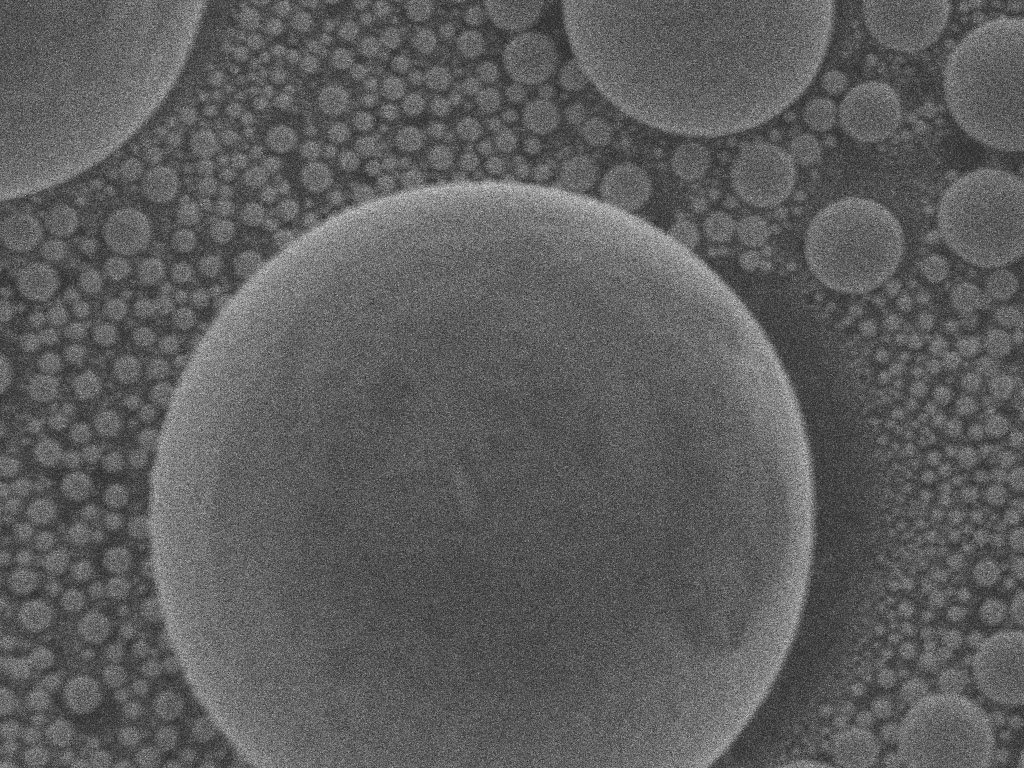
\includegraphics[width=0.3\textwidth]{Images/A in focus.jpg}
        \caption{In focus}
        \label{A in focus}
    \end{subfigure}
    \begin{subfigure}{\textwidth}
        \centering
        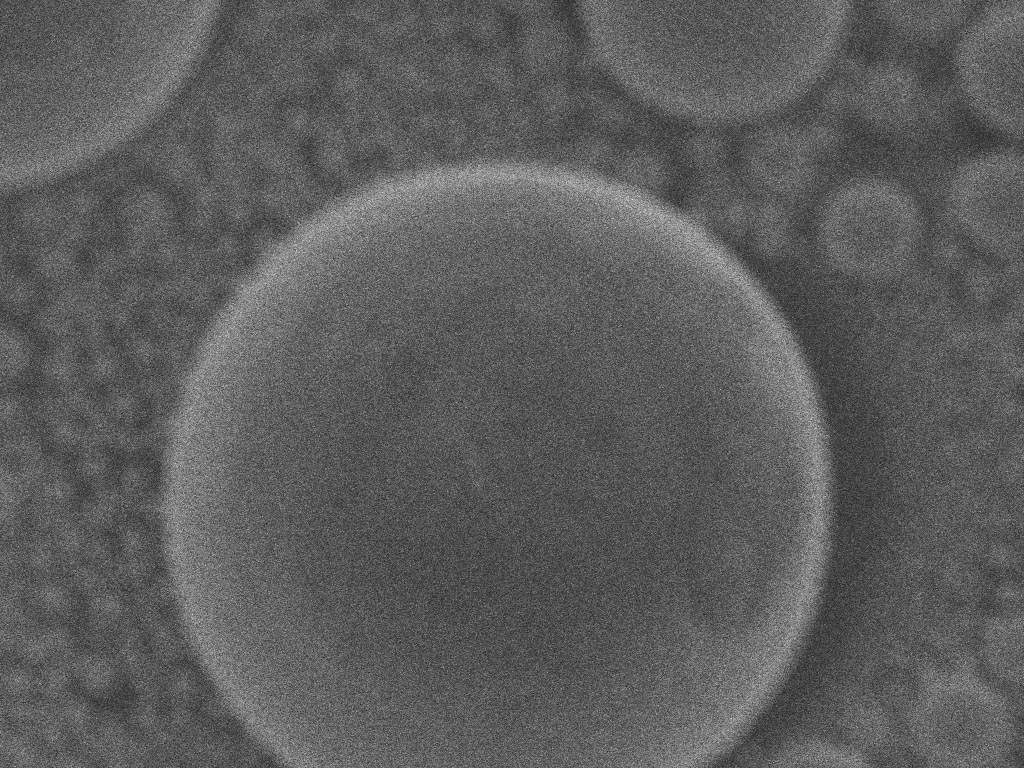
\includegraphics[width=0.3\textwidth]{Images/A out of focus.jpg}
        \caption{Out of focus}
        \label{A out of focus}
    \end{subfigure}
    \begin{subfigure}{\textwidth}
        \centering
        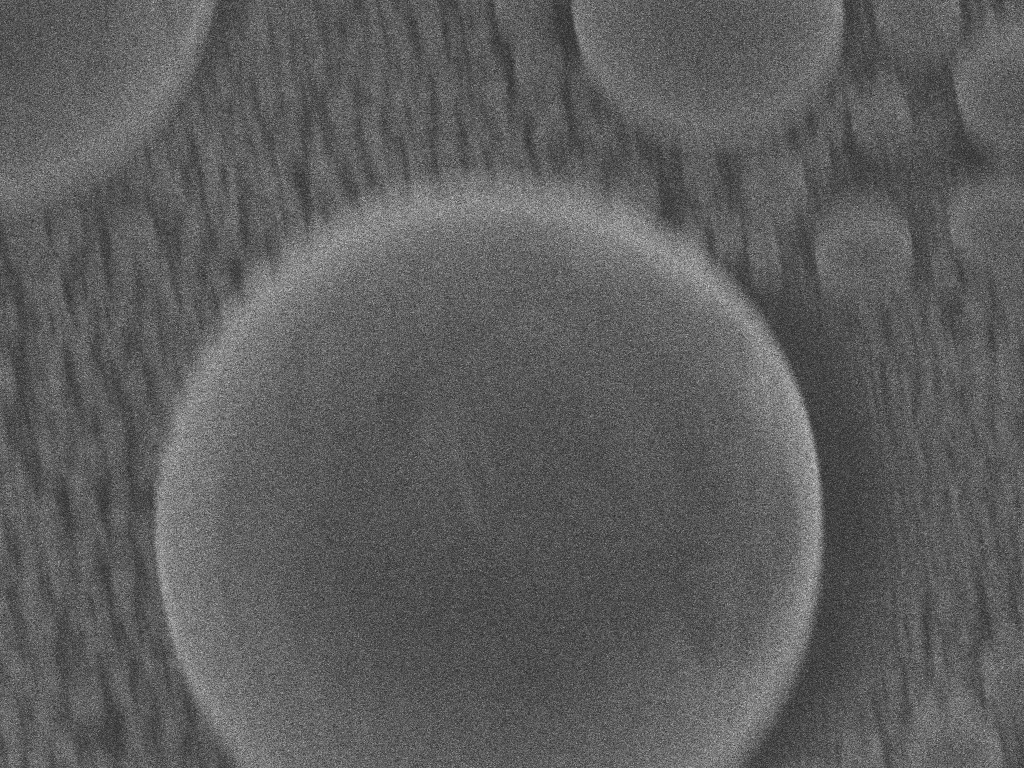
\includegraphics[width=0.3\textwidth]{Images/A astigmatism.jpg}
        \caption{In focus with astigmatism}
        \label{A astigmatism}
    \end{subfigure}
    \caption{Sample SEM images}
    \label{Sample SEM images}
\end{figure}

Although experienced SEM operators can often find the right settings for focus and stigmatism in a short time, it may not be as straightforward for new users. Sometimes, the surface being observed may have a complex structure and makes adjusting even harder. The complexity arises because any judgement of an image is based on what the operators see through their eyes, which is rather subjective. Intensive training and practical experience are often required for an operator to become efficient in using the SEM.

Fast computing can aid the operators in a few ways. Firstly, a numerical evaluation of the quality of the image may be provided, which eliminates the subjectivity in using human eyes. Numbers are also easier to note down if any record is required. Two operators may have different views on the same image, but the numbers will not be different. Therefore, cooperation and communication between operators can be enhanced. The use of numbers also enable automatic procedures for adjusting settings of the SEM, which save time and may produce better results than doing it manually.

The project focuses on developing tools that use Fast Fourier Transform (FFT) to help operators evaluate the focusing and astigmatism of SEM images, and also looks into an algorithm for the automatic correction of them.

\section{The Algorithms}
\subsection{Histogram Equalisation}
The idea of histogram.
The maths of histogram.
Demonstration of the algorithm.
Speed test of the algorithm.

\subsection{Fast Fourier Transform} 
Idea of FT.
Maths of FFT.
Demonstration.
Speed test. 

\subsection{Focusing and Astigmatism Correction}
Idea.
Algorithm and flow chart.
Demonstration of current result.
Next step.

\section{The Software}
\subsection{Overview}
Overview of all modules.

\subsection{The SemImage Module}
Idea of the module.
Classes and functions.
Demo code.
Possible improvements.

\subsection{The SemTool Module}
Idea of the module.
Classes and functions.
Demo code.
Possible improvements.

\subsection{The SemCorrector Module}
Idea of the module.
Classes and functions.
Demo code.
Possible improvements.

\section{Demonstrations}
\subsection{Real-time Histogram Equalisation}
Screenshots of the software.

\subsection{Real-time Fast Fourier Transform}
Screenshots of the software.

\subsection{Automatic Focusing and Astigmatism Correction}
Screenshots of the software.
Test results.

\section{Next Steps}
Next steps.

\newpage
\begin{thebibliography}{}
    \bibitem{SEM A to Z}
    \textit{Scanning Electron Microscope A to Z}. JEOL Ltd. [Online]. Available: \url{https://www.jeol.co.jp/en/applications/pdf/sm/sem_atoz_all.pdf}. Accessed: May 9, 2020.

    \bibitem{SEM for semiconductor}
    T. Agemura and T. Sekiguchi, "Secondary electron spectroscopy for imaging semiconductor materials," 2018 International Symposium on Semiconductor Manufacturing (ISSM), Tokyo, Japan, 2018, pp. 1-3, doi: 10.1109/ISSM.2018.8651171.
    
    \bibitem{SEM wiki}
    "Scanning electron microscope." en.wikipedia.org. \url{https://en.wikipedia.org/wiki/Scanning_electron_microscope} (accessed May 9, 2020).
\end{thebibliography}
\end{document}
